\chapter{Path Tracing}
\label{chaper:PathTracing}
In this chapter we show how to express the rendering equation over path space and represent the light transport problem without any recursions. This formulation lets us design a basic path tracing algorithm, where we create random paths to approximate the rendering equation. We will outline some sampling strategies that are commonly used for path tracing and shortly introduce our new approach for sampling incident radiance. These strategies have different effects on the quality of the resulting images and can be combined using Multiple Importance Sampling. Last we will introduce Russian Roulette as a method to reduce computation time.

\section{Path Space}

First, we need to define paths and path space:
\begin{itemize}
\item $x=x_0x_1\dots x_k$ is a path with length $1 \leq k < \infty$ defined by surface points $x_i$ \\
\item $\Omega_k$ is the set of all paths of length $k$\\
\item $\mu_k(D) = \int\limits_DdA(x_0) \cdots dA(x_k)$ is the \emph{area-product measure} on $\Omega_k$, with $D\subseteq \Omega_k$
\item $\Omega = \bigcup\limits_{k=1}^\infty \Omega_k$ is the \emph{path space}. It contains all paths with a finite length.
\item $\mu(D) = \sum\limits_{k=1}^\infty \mu_k(D\cap \Omega_k)$ is the area-product measure for $\Omega$
\end{itemize}

\section{Rendering Equation over Path Space}

We will now expand the three-point form of the rendering equation one step. Since the terms will get very long, we will abbreviate $L(a \rightarrow b)$, $f_s(a \rightarrow b \rightarrow c)$ and $G(a \leftrightarrow b)$ with $L(a,b)$, $f_s(a,b,c)$ and $G(a,b)$.

\begin{align*}
L(x_1\rightarrow x_0) &= L_e(x_1,x_0) + \int_\mathcal{M}L(x_2, x_1) f_s(x_2, x_1,  x_0) G(x_2, x_1) dA(x_2)\\
&=  L_e(x_2, x_1) + \int_\mathcal{M}\left( L_e(x_2,x_1) + \int_\mathcal{M}L(x_3 , x_2) f_s(x_3 , x_2, x_1) G(x_3 , x_2) dA(x_3) \right)\\ 
&\qquad\qquad\qquad\qquad\qquad \cdot  f_s(x_2,x_1, x_0) G(x_2, x_1) dA(x_2)\\
&= L_e(x_1,x_0) + \int_\mathcal{M}L_e(x_2 , x_1) f_s(x_2 , x_1, x_0) G(x_2,x_1) dA(x_2) +\\
&\qquad \int_{\mathcal{M}^2}L(x_3 , x_2) f_s(x_3, x_2, x_1) G(x_3 ,x_2)\\
&\qquad\qquad\qquad \cdot f_s(x_2, x_1 , x_0) G(x_2 , x_1) dA(x_2)dA(x_3).\\
\end{align*}

If we continue to do this and merge the result with the measurement equation \ref{measurement equation}, we can rewrite $I^j$ with $x_0$ on pixel $j$ as

\begin{equation*}
\begin{split}
I^j=\sum_{k=1}^\infty &\int_{\mathcal{M}^{k+1}}L_e(x_k \rightarrow x_{k-1})G(x_k \leftrightarrow x_{k-1}) \\
&\qquad\cdot\left(  \prod_{i=1}^{k-1} f_s(x_{i+1} \rightarrow x_i \rightarrow x_{i-1}) G(x_i \leftrightarrow x_{i-1}) \right)\\
&\qquad\cdot W_e^j(x_1 \rightarrow x_0) dA(x_0) \cdots dA(x_k).
\end{split}
\end{equation*}


Since we have removed any $L_i$ and $L_o$ from the equation, we can now solve $I^j$ without any recursion by evaluating all the integrals. The integrand is defined for each path length and gives us the \emph{measurement contribution function}

\begin{equation}
\label{mcf}
\begin{split}
f_j(x) &= L_e(x_k \rightarrow x_{k-1}) G(x_k \leftrightarrow x_{k-1}) \cdot\\
& \qquad \left( \prod_{i = 1}^{k-1} f_s(x_{i+1} \rightarrow x_i \rightarrow x_{i-1}) G(x_{i} \leftrightarrow x_{i-1}) \right) W_e^j(x_1 \rightarrow x_0).
\end{split}
\end{equation}

Figure \ref{transportpath} shows an example for a transport path $x_0\dots x_4$ with all relevant factors.\\
\begin{figure}[ht]
	\centering
\def\svgwidth{400pt}
  \input{transportpath.pdf_tex}
\caption{A possible light transport path $x_0x_1x_2x_3x_4$ with all factors for the measurement contribution function.}
\label{transportpath}\end{figure}
We can now compute $I^j$ with the \emph{path integral} as follows:

\begin{equation}
\label{path integral}
I^j=\int_\Omega f_j(x)d\mu(x).
\end{equation}

This formulation allows us to evaluate the color of a pixel without any recursions by integrating over path space. However, as the path space has a theoretically infinite number of dimensions, we apply Monte Carlo integration to solve the path integral.


\begin{equation}
\label{path integral estimator}
\int_{\Omega}f_j(x)d\Omega(x) = E\left(\frac{f_j(X)}{p(X)}\right) \approx \frac{1}{N}\sum_{i=1}^N \frac{f_j(X_i)}{p(X_i)}
\end{equation}

where $p(X)$ is a probability density function for sampling a certain path measured over surface areas, and $X$ was sampled according to $p$.

What we have to do next is create $N$ paths of any length, compute their probability and their contribution and weight them together. The next part will cover how to find a good pdf in order to decrease the variance of our estimate. After that we show the basic structure of a path tracing algorithm.








\section{Importance Sampling Options}
\label{importance_sampling_options}

Since we build paths by separately creating one point after another, starting from the camera, we can only affect three factors of the total path integral at each point $x_i$ where we have to extend the path. We can directly influence the values of $f_s(x_{i+1} \rightarrow x_i \rightarrow x_{i-1})$ and the $cos(x_i \rightarrow x_{i+1})$ part of $G(x_i \leftrightarrow x_{i+1})$ (at least as long as we don't include the cosine at the next potential path point $x_{i+1}$) when we sample $x_{i+1}$. But we can also try to choose path directions that lead us to a a high $L_e$ fast, so that we lose as little energy as possible while traversing the scene.

So instead of one sampling strategy that yields one pdf for the whole path integral, we will create a new pdf at each point $x_i$ locally and only use it once to sample the next point $x_{i+1}$ until we hit a light source or sample a direction that leaves the scene. It is therefore sufficient to simply consider the scattering equation for the current path point $x$ when we want to pick a pdf.\\
There are several options for choosing pdfs that are roughly proportional to the integrand in the scattering equation \ref{scattering equation}

\begin{equation}
\label{scattering solid}
\begin{split}
L_{o,s}(x,\omega) &= \int_{\mathcal{S}^2}  L_i(x,\omega_i) \cdot f_s(\omega_i,x,\omega_o) d\sigma^\bot(\omega_i)\\
 &= \int_{\mathcal{S}^2}L_i(x,\omega_i) \cdot f_s(\omega_i,x,\omega_o) \cdot cos(w_i) d\sigma(w_i).
\end{split}
\end{equation}

Obviously, the integrand will get bigger for bigger $f_s$, $L_i$ and cosine values, although a big cosine can always be cancelled by a small BSDF value or relatively little irradiance (and the other way around).
Generally most pdfs try to approximate only one of the factors $f_s$, $L_i$ or $cos(\omega_i)$.

The next few segments will outline four pdf choices and address their strengths and weaknesses. All options offer certain benefits under certain circumstances, but also show substantial flaws under others. Therefore it is common to combine different strategies (usually BSDF sampling and next event estimation) in order to perform well under any condition. 

\subsection{Cosine to normal}
The plainest option is to generate samples proportional to their cosine with the surface normal. Many samples will be roughly perpendicular to the surface and less will follow flat directions.\newline
Unfortunately, as the pdf is basically just a scaled cosine function, it doesn't necessarily approximate the full integrand very well. For example, the more specular the BSDF, the more the value of the integrand depends on $\omega_o$ and $f_s$. Another potential problem is strong but flat radiance with almost no radiance from above, as most samples will be far away from flat directions.\newline
Theoretically, this pdf will produce correct results in any case if enough samples are used, but this may take way longer than the other options proposed below.

\subsection{BSDF sampling}
Next we discuss a pdf that is proportional to the BSDF and will lead to more samples wherever $f_s$ is big. If the probabilities are expressed over solid angle we can apply formulation \ref{scattering solid} of the scattering equation. This enables us to use Monte Carlo integration to approximate the scattering integral with a pdf $p \propto f_s$ as follows:
\begin{equation}
\int_{\mathcal{S}^2} L_i(x,\omega_i) \cdot f_s(\omega_i,x,\omega_o) \cdot cos(\omega_i)d\sigma(\omega_i)\approx \frac{L_i(x,\omega_i') \cdot f_s(\omega_i',x,\omega_o) \cdot  cos(\omega_i')}{p(\omega_i')},
\end{equation}

where $\omega_i'$ is a random variable with density $p$ measured over solid angle.

This strategy can be repeated to approximate $L_i(x,\omega_i')$ in turn until a light source is hit. If BSDF sampling is the only strategy used to create a path, we can get the total energy arriving at the camera along that path like this:

\begin{algorithm}
\caption{basic path tracing with BSDF only}
\begin{algorithmic}[1]
\State $j \gets 1$
\State create Camera ray with direction $-\omega_o^j$
\State $x_j \gets$ first intersection of ray with scene
\State $pathEnergyWeight \gets W_e^j(x_1 \rightarrow x_0) \cdot G(x_1 \leftrightarrow x_0) / p_A(x_1)$
\While {$x_j$ not on light source}
\State $\omega_i^j \gets $ new sample from surface BSDF at $x_j$
\State $pathEnergyWeight \gets pathEnergyWeight \cdot \frac{f_s(\omega_i^j,x_j,\omega_o^j) \cdot cos(\omega_i^j)}{p(\omega_i^j)}$
\State $j\gets j+1$
\State $x_j \gets $ first intersection of ray along $\omega_i^j $ with scene
\If {no intersection exists}
\State \textbf{return} 
\EndIf
\State $\omega_o^j \gets -\omega_i^j $ 
\EndWhile
\State $k \gets j$
\State $totalEnergy \gets pathEnergyWeight \cdot L_e(x_k,\omega_o^k)$
\end{algorithmic}

\label{weightPath_BSDF}\end{algorithm}

\pagebreak
Note that we terminate any path in line 11 if a ray along the sampled direction doesn't intersect the scene, as well as we stop each path the first time it hits a light source. Plus, we have to revert the direction in line 13 so we can insert it to $f_s$ when we get to line $7$ again.

We will now recalculate what happens in algorithm \ref{weightPath_BSDF}. In order to abbreviate the next equation, we define
$G_{0,1} := G(x_0 \leftrightarrow x_1)$ and $W:=W_e^j(x_1 \rightarrow x_0)$.\\
Assuming we don't leave the scene and end up with a path $(x_0, \dots, x_k)$ with $x_0$ on the camera and $x_k$ on a light source, the total energy arriving at the camera along that path will be 
\begin{equation}
\begin{split}
totalEnergy &= L_e(x_k,\omega_o^k) \frac{G_{0,1} W}{p_A(x_1)} \cdot \prod_{j = 1} ^{k-1} \frac{f_s(\omega_i^j,x_j,\omega_o^j) \cdot cos_{x_j}(\omega_i^j)}{p(\omega_i^j)}\\
&=  L_e(x_k \rightarrow x_{k-1})  \frac{G_{0,1} W}{p_A(x_1)} \cdot \prod_{i=1}^{k-1} \frac{f_s(x_{i+1} \rightarrow x_i \rightarrow x_{i-1}) \cdot cos(x_i \rightarrow x_{i+1})}{p(x_i \rightarrow x_{i+1})}\\
&= L_e(x_k \rightarrow x_{k-1})  \frac{G_{0,1} W}{p_A(x_1)} \cdot \prod_{i=1}^{k-1} \frac{f_s(x_{i+1} \rightarrow x_i \rightarrow x_{i-1}) \cdot G(x_i \leftrightarrow x_{i+1})}{p_A(x_{i+1})}.\\
\end{split}
\end{equation}

$cos(x \rightarrow y)$ represents the cosine of the surface normal at $x$ with the direction of a ray from $x$ through $y$. $p_A$ is $p$ converted to the surface area measure (see equation \ref{geotrans}).\\
The last line is equivalent to the measurement contribution function \ref{mcf} divided by the probability of sampling $x_0\dots x_k$. This result can now be added to our estimator \ref{path integral estimator}.\\

\textbf{Strengths and Weaknesses}

Samplig the BSDF works especially well for highly specular surfaces, but shows weaknesses when dealing with small light sources.\newline
Whenever a surface is highly specular, the BSDF strongly determines where the integrand can even reach big values, regardless of the actual irradiance. On the other hand, if a surface is ideally diffuse, the BSDF has no influence whatsoever on the integrand's magnitude. In that case, sampling the BSDF would be no better than generating directions completely at random. Figure \ref{BSDF_veach} shows how the roughness of a surface and the size of a light source determine the quality of BSDF sampling.


 \begin{figure}[ht]
 \centering
 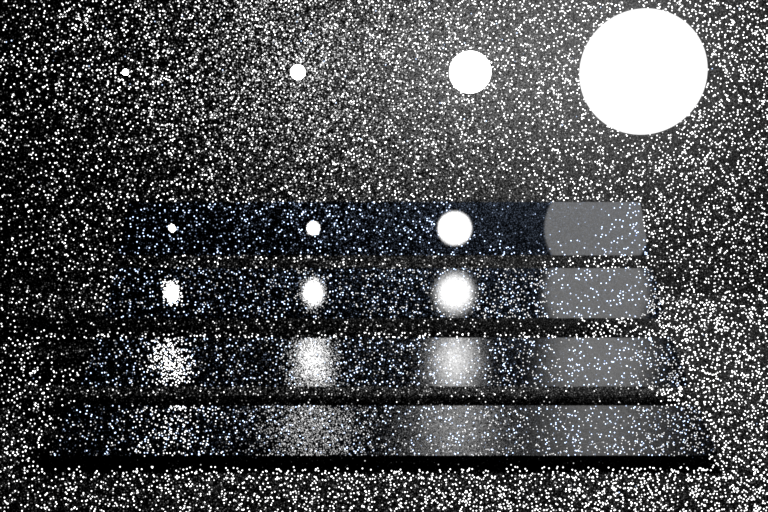
\includegraphics[width=0.52\textwidth]{bilder/veach/bsdf_64.png}
 \caption{On the upper right, where the surface is highly specular and the light sources are large, BSDF sampling performs rather well.\newline
On the lower left as well as the floor and wall, where the surface is highly diffuse and the light sources are small, BSDF sampling produces a lot of noise.}
  \label{BSDF_veach}\end{figure}



A problem with generating samples solely from the BSDF is that the path is not very likely to hit a light source. This leads to more longer paths and, when the scene is not closed, to paths completely leaving the geometry. The smaller the area covered by light sources the more paths will be leaving the scene before hitting a light source. Figure \ref{BSDFsampling_spp} shows how BSDF sampling behaves for different numbers of samples per pixel.
 
 Additional properties of BSDF sampling (as well as next event estimation) can be found in \cite{veachdiss}.


 \begin{figure}[ht!]
 \centering
 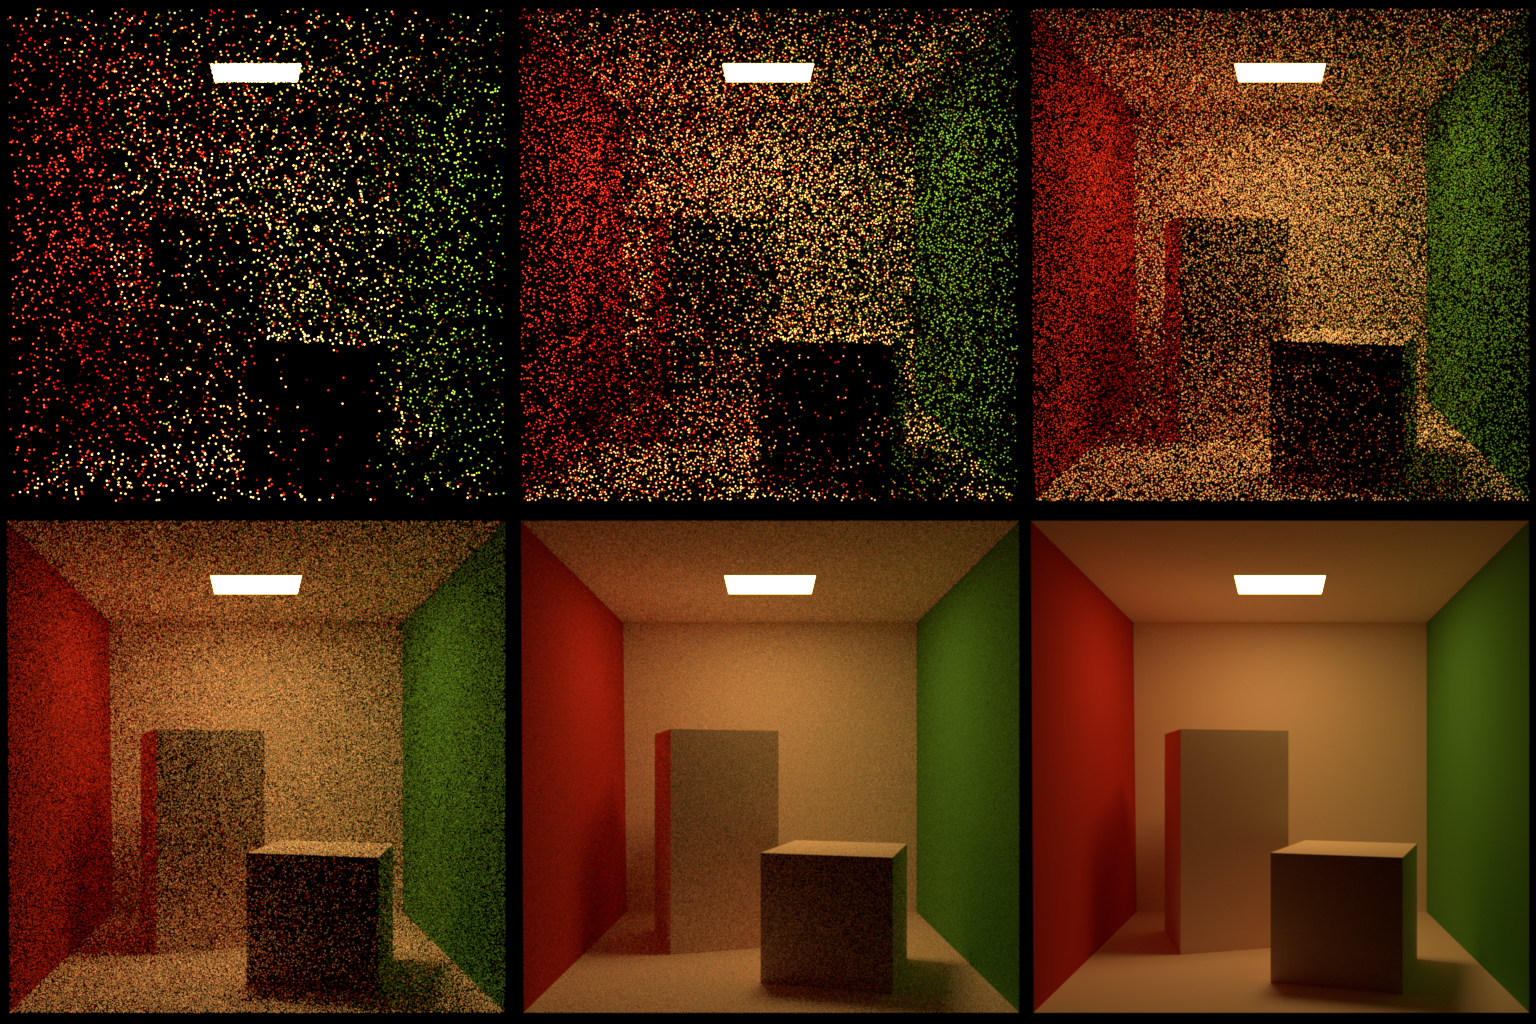
\includegraphics[width=1\textwidth]{bilder/bsdf_sampling/1-4-16-64-1024-mts.png}
 \caption{BSDF sampling with 1, 4, 16, 64 and 1024 samples per pixel, and a perfect image on the bottom right (created with another algorithm).\newline
Note how even 1024 samples per pixel still produce some noise compared to the exact solution.}
  \label{BSDFsampling_spp}\end{figure}


\subsection{Next Event Estimation}
As seen above, sampling the BSDF shows some flaws when dealing with diffuse surfaces and small light sources. Next Event Estimation (NEE) is a sampling strategy that performs by far better in these cases, but exhibits some weaknesses for specular surfaces and large light sources.\newline
With NEE, samples are not generated as outgoing directions at the surface point in order to create paths of arbitrary length, but as points on any light source instead: We take an incomplete path $(x_0,\dots,x_k)$, sample a point $x'$ on a light source and check if $x_k$ and $x'$ are visible to each other. If that's the case we have created a complete path from the camera ($x_0$) to a light source ($x'$). Since this strategy always terminates the given path, using it exclusively would result in creating mainly short paths. As a consequence NEE is usually combined with BSDF sampling.

The goal of this strategy is to use a pdf that approximates $L_i(x,\omega_i)$. Since most surface interactions attenuate the energy of incoming light, $L_i$ will presumably be a lot bigger if $\omega_i$ points directly to a light source.

In order to better understand how a pdf for NEE can be created, we look at the scattering integral over surface area. Remember the three-point form of the rendering equation \ref{tpf}, where we included a geometry term $G$ in order to compensate for the conversion from solid angle to surface area:

\begin{equation*}
L_o(x' \rightarrow x'') = \int_\mathcal{M} L(x \rightarrow x') f_s(x \rightarrow x' \rightarrow x'') G(x\leftrightarrow x')dA(x).
\end{equation*}

Now, intuitively $L(x \rightarrow x')$ will be a lot bigger whenever $x$ is actually emitting light instead of just redirecting and thereby attenuating it. As we have no analytical information on $L$ (as opposed to sampling the BSDF or cosine), we use the alternative approximation of giving a high probability to those $x$ on light sources. When combining NEE and BSDF, the multi-sample model even allows for this pdf to be $0$ for all points that are not part of a light source.

Usually a light source is picked according to its area and intensity, and a point on that light source is sampled uniformly. These probabilities are initially measured over surface area and have to be converted to solid angle, if we want to combine NEE and BSDF sampling.\\

\textbf{Strengths and Weaknesses}

As indicated above, NEE performs well for small light sources as well as highly diffuse surfaces. Veach illustrates the different aspects of NEE versus BSDF sampling with the glossy highlights problem in \cite[chapter 9.3.1]{veachdiss}. We used a replica of his scene from the Mitsuba download website \cite{mitsuba}. The results are shown in figure \ref{veach_mis} for BSDF sampling, NEE and the combination of both using the multi-sample model.\\
The biggest problem with NEE is that it completely ignores strong indirect lighting (e.g. from mirrors or glass surfaces) and can therefore not render any caustics (see figure \ref{nee_caustics}).

 \begin{figure}[ht]
 \centering
 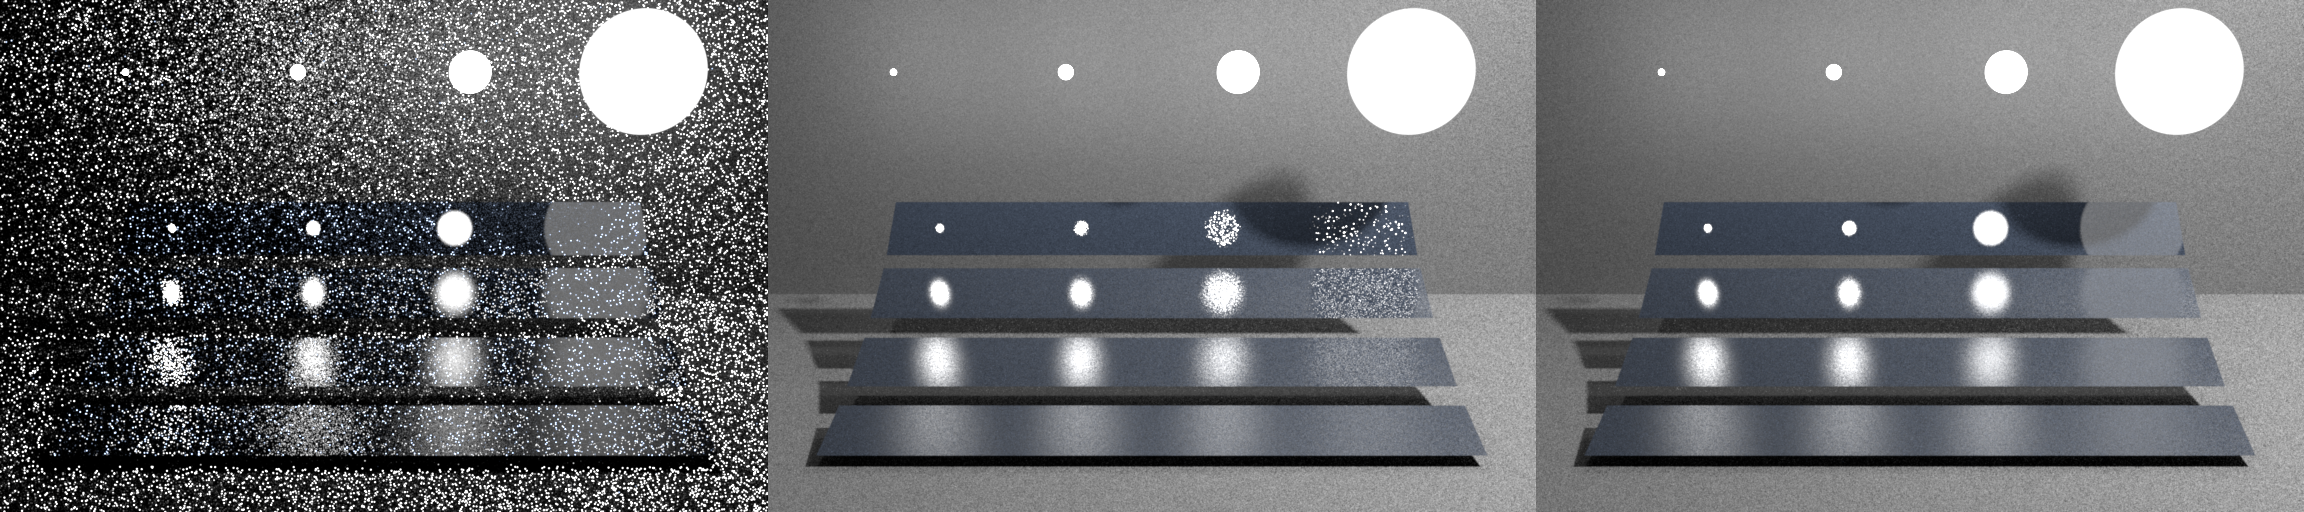
\includegraphics[width=1\textwidth]{bilder/veach/bsdf_nee_beids_64.png}
\caption{Left: BSDF sampling (good with specular surfaces and large light sources)\newline
Center: NEE (good with small light sources or diffuse surfaces)\newline
Right: MIS of BSDF sampling and NEE}
 \label{veach_mis}\end{figure}



 \begin{figure}[ht]
 \centering
 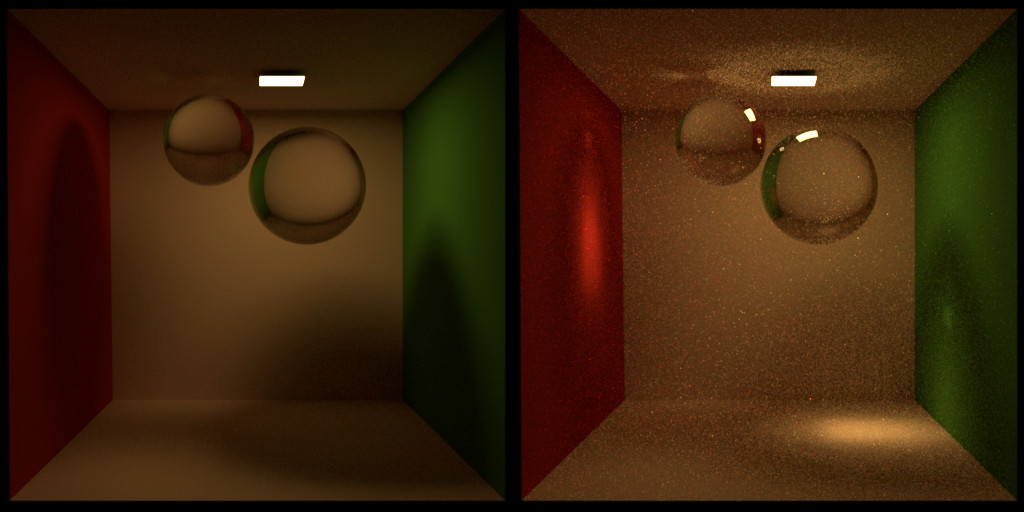
\includegraphics[width=0.8\textwidth]{bilder/kugelbox/nee_caustics.png}
\caption{Left: NEE only, the caustics are missing. Right: Reference with caustics.}
  \label{nee_caustics}\end{figure}



\subsection{Irradiance Sampling}
The main part of this thesis will cover caches for incident radiance as an alternative way to create a pdf proportional to $L_i$. While NEE only considers direct illumination and can be computed as needed, our approach to irradiance sampling requires a preprocessing step. In that step, the incident radiance - direct and indirect - is approximated and cached. Each cache is placed at a surface point $x$ and provides a pdf that is proportional to the incident radiance arriving at $x$ from different directions. The pdf values are measured over solid angle. As shown later, sampling an outgoing direction from such a cache is fast and simple, and - given certain conditions - irradiance importance sampling can offer advantages over NEE or BSDF sampling.\newline
In chapter \ref{chapter:irradiance_caching} we show how we used caches to approximate incident radiance, and chapter \ref{chapter:rendering} will explain how to use these caches for irradiance importance sampling.




\section{Path contribution}

Assuming that we have created a path $x = x_0x_1\dots x_k$ according to some strategy, we can now compute its contribution to our estimator from equation \ref{path integral estimator} as

\begin{equation*}
contribution(x) = \frac{f_j(x)}{p(x)}.
\end{equation*}

The total probability of sampling the whole path is given as the product of all probabilities used to sample a new point of the path. We only use forward sampling, meaning that we only sample new points on a path from camera to light source. Note that bidirectional techniques use both forward and backward sampling - subpaths are sampled starting both from a light source and from the camera, which affects the way their probabilities have to be computed. See \cite[chapter 10]{veachdiss} for further information.

Note that equation \ref{path integral} is measured by the area-product measure. So theoretically we have to measure our probabilities over surface area. Let $p_A(x_{i+1})$ be the probability of sampling (the direction to) $x_{i+1}$ when we are at point $x_i$, measured over surface area, and let $p_\sigma(x_i \rightarrow x_{i+1})$ be the probability of sampling $x_{i+1}$ from $x_i$ measured over solid angle. We can convert between $p_A$ and $p_\sigma$ similar to equation \ref{geotrans} as follows:

\begin{equation}
\label{pdftrans}
p_A(x_{i+1}) \cdot cos(x_i \rightarrow x_{i+1}) = G(x_i \leftrightarrow x_{i+1}) p_\sigma(x_i \rightarrow x_{i+1}),
\end{equation}

In the next equation we will replace $f_s(a \rightarrow b \rightarrow c)$ with $f_s(a,b,c)$ and $G(a \leftrightarrow b)$ with $G(a,b)$, and we will use

\begin{equation*}
W :=  \frac{W_e^j(x_1 \rightarrow x_0) G(x_0,x_1)}{p_A(x_1)}.
\end{equation*}

The total contribution of a path $x=x_0x_1\dots x_k$ from camera to light can be computed by combining $p$ and $f_j$.
\pagebreak
\begin{equation}
\label{geoweg}
\begin{split}
contribution(x) &= L_e(x_k \rightarrow x_{k-1}) \cdot W \cdot \prod _{i=1}^{k-1} \frac{f_s(x_{i+1},x_i, x_{i-1}) G(x_i, x_{i+1})}{p_A(x_{i+1})}\\
&= L_e(x_k \rightarrow x_{k-1}) \cdot W \cdot \prod _{i=1}^{k-1} \frac{f_s(x_{i+1},x_i, x_{i-1}) cos (x_i \rightarrow x_{i+1})}{p_\sigma(x_i \rightarrow x_{i+1})}.
\end{split}
\end{equation}

Equation \ref{geoweg} shows that the geometry term disappears almost completely if we measure our pdfs over solid angle. Fortunately this is also way more convenient for BSDF sampling and our caches, as these strategies only provide directions and don't make use of any information on the other surfaces in the scene - the next path point is only retrieved by casting a ray from the current path point along the sampled direction.

This also means that we can assemble the path's contribution gradually while we create it, as depicted in algorithm \ref{assembleenergy}: At each point $x_i$ we evaluate the local BSDF for the previous and sampled direction and the cosine factor for the sampled direction. We multiply these values together, and as soon as we hit a light source we multiply $L_e$ and are done.

\begin{algorithm}
\caption{Assemble a path's energy}
\label{assembleenergy}
\begin{algorithmic}
\State $weight \gets W$
\While {$x_i$ not on light source}
\State Sample $x_{i+1}$
\State $weight \gets weight \cdot \frac{f_s(x_{i+1},x_i,x_{i-1}) cos(x_i \rightarrow x_{i+1})}{p_\sigma(x_i \rightarrow x_{i+1})}$
\EndWhile
\State \textbf{return} $L_e(x_k \rightarrow x_{k-1}) \cdot weight$
\end{algorithmic}
\end{algorithm}



Note that for NEE, where we sample a point instead of a direction, a pdf measured over surface area is more convenient. So if we hit the light source deliberately by using NEE, we need to replace the last $\frac{cos(x_{k-1} \rightarrow x_k)}{p_\sigma(x_{k-1} \rightarrow x_k)}$ with $\frac{G(x_{k-1} \leftrightarrow x_k)}{p_A(x_k)}$.

\newpage
\section{The Algorithm}
\label{pathtracingalgorithm}

Algorithm \ref{weightPath_BSDF} already provided a short example of a basic path tracing algorithm that only used the BSDF to extend paths.

We will now expand that example to include BSDF sampling as well as NEE and add MIS weights according to the multi-sample model. We ignored $W_e^j(x_1 \leftrightarrow x_0)$, $p_A(x_1)$ and $G(x_1 \leftrightarrow x_0)$ in our implementation, since $W_e^j$ is usually defined in a way that all three factors are cancelled out to prevent vignetting.

We use the following notation:
\begin{itemize}
\item $p_{A,nee}(x')$ is the pdf value for sampling a point $x'$ on any light source, measured over surface area. $p_{\sigma,nee}$ is the same pdf measured over solid angle.
\item Given points $x_1, x_2$ and $x_3$, $p_{BSDF}(x_3)$ is the probability of sampling the incident direction $x_3 - x_2$ from the local BSDF at $x_2$ with outgoing direction $x_1 - x_2$.
\end{itemize}
We use the power heuristic \ref{power heuristic} to weight NEE and BSDF sampling together. A similar algorithm can be found in \cite{survey}. 

\begin{algorithm}
\caption{Path tracing with BSDF sampling and NEE}
\label{ptBSDF}
\begin{algorithmic}[1]

\State $x_0 \gets $ point on Camera
\State $\omega_1 \gets $ first ray direction

\State $x_1 \gets x_\mathcal{M}(x_0,\omega_1)$
\State $w_{BSDF} \gets 1$
\State $i \gets 1$
\State $throughput \gets 1$
\State $color \gets black$
\While {true}
\If {$L_e(x_i \rightarrow x_{i-1}) > 0$}
\State \textbf{return} $throughput  \cdot w_{BSDF} \cdot L_e(x_i \rightarrow x_{i-1}) + color$

\Else

\State
\State $x' \gets samplePointOnLightSource()$
\If {$x'$ is visible from $x_i$}
\State $w_{nee} \gets \frac{p_{\sigma,nee}(x')^2}{p_{\sigma,nee}(x')^2 + p_{BSDF}(x')^2}$
\State $L \gets L_e(x' \rightarrow x_i)$
\State $color \gets color + L \cdot throughput \cdot w_{nee} \cdot f_s(x' \rightarrow x_i \rightarrow x_{i-1}) \cdot \frac{G(x_i \leftrightarrow x')}{p_{A,nee}(x')}$

\EndIf
\State
\State $\omega_{i+1} \gets $ bsdf.sampleDirection$(x_i,\omega_i)$

\If {$ray(x_i,\omega_{i+1})$ intersects scene}
\State $x_{i+1} \gets x_\mathcal{M}(x_i,\omega_{i+1})$
\State $throughput \gets throughput \cdot f_s(x_{i+1} \rightarrow x_i \rightarrow x_{i-1})\cdot \frac{cos(x_i \rightarrow x_{i+1})}{p_{BSDF}(x_{i+1})}$
\State $w_{BSDF} \gets \frac{p_{BSDF}(x_{i+1})^2}{p_{BSDF}(x_{i+1})^2 + p_{\sigma,nee}(x_{i+1})^2}$
\Else
\State \textbf{return} $color$

\EndIf

\State $i \gets i+1$
\EndIf
\EndWhile

\end{algorithmic}
\end{algorithm}
\pagebreak


This algorithm usually creates multiple paths: One so-called ``implicit path'', where we continue to sample points from the BSDF until we accidentally hit a light source, and several ``explicit paths'' that are created by deliberately sampling a point on the light source. However, since we terminate any path as soon as it hits a light source, we always extend exactly one path. The explicit paths are terminated as soon as they are created and pose no problem in terms of an exponentially growing number of paths to pursue.






\section{Russian Roulette}
\label{chapterRussianRoulette}
In an enclosed environment, paths generated by BSDF sampling can get arbitrarily long before reaching a light source. Not only do these paths carry very little energy, they also take much more time to compute. Russian Roulette is a common solution to achieve better computing time while not manipulating the correct solution by ignoring these paths completely.

With Russian Roulette, all paths are randomly terminated after reaching a certain length: Every time before the path is extended, a random number $r$ is compared to a threshold $\alpha \in \lbrack 0,1\rbrack$. If $r>\alpha$, the path is terminated. If $r \leq \alpha$, the path is continued and weighed with $\frac{1}{\alpha}$. As a result, there will be fewer but more heavily weighted long paths and more short paths with smaller weights. As this approach still explores all possible paths it still generates a correct solution.

Too small $\alpha$ values can lead to an extremely low number of long paths, that in exchange are extremely highly weighted and result in fireflies in the final image. On the other hand, Russian Roulette will rarely cancel any paths at all, if $\alpha$ is constantly too big. Usually $\alpha$ is determined dynamically, depending on criteria such as the path's current length, its contribution or surface properties (e.g. reflectance).\\
Since very short paths will almost always be important to a pixel's color, Russian Roulette should only be applied to paths above a certain length.

However, Russian Roulette will always lead to a higher variance, so we only applied it to paths with a length over $20$.
